
\begin{figure}
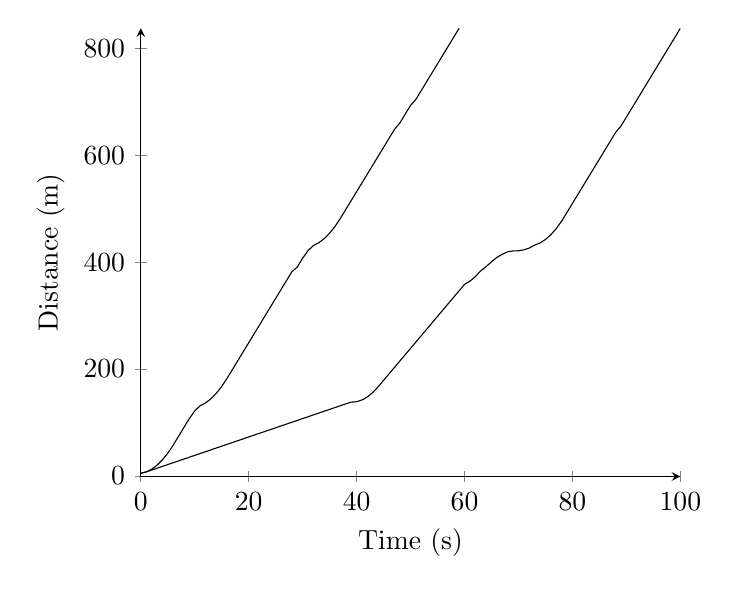
\begin{tikzpicture}
\begin{axis}[
legend style={anchor=west},
axis x line=bottom,
axis y line=left,
ymin=-1,
xlabel=Time (s),
ylabel=Distance (m),
]
\addplot[] coordinates {
(0, 5.1)
(1, 7.6)
(2, 12.6)
(3, 20.1)
(4, 30.1)
(5, 42.6)
(6, 57.6)
(7, 74.2)
(8, 90.8)
(9, 107.4)
(10, 121.758781889)
(11, 131.320742477)
(12, 136.609280481)
(13, 144.397818486)
(14, 154.68635649)
(15, 167.474894495)
(16, 182.763432499)
(17, 199.363432499)
(18, 215.963432499)
(19, 232.563432499)
(20, 249.163432499)
(21, 265.763432499)
(22, 282.363432499)
(23, 298.963432499)
(24, 315.563432499)
(25, 332.163432499)
(26, 348.763432499)
(27, 365.363432499)
(28, 381.963432499)
(29, 390.693432499)
(30, 407.293432499)
(31, 421.530003602)
(32, 430.979274031)
(33, 436.172518048)
(34, 443.865762065)
(35, 454.059006083)
(36, 466.7522501)
(37, 481.945494117)
(38, 498.545494117)
(39, 515.145494117)
(40, 531.745494117)
(41, 548.345494117)
(42, 564.845494117)
(43, 581.445494117)
(44, 598.045494117)
(45, 614.645494117)
(46, 631.245494117)
(47, 647.845494117)
(48, 659.985494117)
(49, 676.585494117)
(50, 693.185494117)
(51, 704.535494117)
(52, 721.135494117)
(53, 737.735494117)
(54, 754.335494117)
(55, 770.935494117)
(56, 787.535494117)
(57, 804.135494117)
(58, 820.735494117)
(59, 837.335494117)
};
\addplot[] coordinates {
(0, 5.1)
(1, 7.6)
(2, 11.0403836148)
(3, 14.4807753176)
(4, 17.9211757371)
(5, 21.3615855687)
(6, 24.8020055841)
(7, 28.2424366415)
(8, 31.6828796988)
(9, 35.1233358275)
(10, 38.5638062312)
(11, 42.0042922659)
(12, 45.444795465)
(13, 48.8853175696)
(14, 52.3258605646)
(15, 55.7664267235)
(16, 59.2070186621)
(17, 62.6476394063)
(18, 66.0882924754)
(19, 69.5289819872)
(20, 72.9697127913)
(21, 76.4104906393)
(22, 79.8513224052)
(23, 83.2922163742)
(24, 86.7331826248)
(25, 90.1742335442)
(26, 93.6153845305)
(27, 97.0566549718)
(28, 100.498069633)
(29, 103.939660668)
(30, 107.381470618)
(31, 110.823557003)
(32, 114.265999615)
(33, 117.708912576)
(34, 121.152465313)
(35, 124.596921342)
(36, 128.042715948)
(37, 131.490629248)
(38, 134.942235443)
(39, 138.105923275)
(40, 138.888910869)
(41, 142.171898463)
(42, 147.954886057)
(43, 156.237873651)
(44, 167.020861245)
(45, 178.980924449)
(46, 190.941229397)
(47, 202.901810585)
(48, 214.8627094)
(49, 226.823975929)
(50, 238.78567138)
(51, 250.747871339)
(52, 262.710670262)
(53, 274.674187756)
(54, 286.638577546)
(55, 298.604040571)
(56, 310.570844626)
(57, 322.539354689)
(58, 334.510081402)
(59, 346.483761811)
(60, 358.461500487)
(61, 364.315031281)
(62, 372.767007777)
(63, 383.718984272)
(64, 391.527928628)
(65, 400.693928308)
(66, 408.755708589)
(67, 414.640830455)
(68, 419.241223761)
(69, 420.923507973)
(70, 421.154886647)
(71, 423.000880674)
(72, 426.366667416)
(73, 431.853575404)
(74, 435.837417107)
(75, 442.32125881)
(76, 451.305100513)
(77, 462.788942217)
(78, 476.77278392)
(79, 493.256625623)
(80, 509.856625623)
(81, 526.456625623)
(82, 543.056625623)
(83, 559.656625623)
(84, 576.156625623)
(85, 592.756625623)
(86, 609.356625623)
(87, 625.956625623)
(88, 642.556625623)
(89, 654.696625623)
(90, 671.296625623)
(91, 687.896625623)
(92, 704.496625623)
(93, 721.096625623)
(94, 737.696625623)
(95, 754.296625623)
(96, 770.896625623)
(97, 787.496625623)
(98, 804.096625623)
(99, 820.696625623)
(100, 837.296625623)
};

\end{axis}
\end{tikzpicture}
\label{tik:distance:100:69}
\caption{100 percent diving with GSC on route $69$}
\end{figure}
